\documentclass{article}
\usepackage{tikz}
\usetikzlibrary{positioning}
\usetikzlibrary{shapes.geometric}
\usetikzlibrary{shapes.symbols}
\usetikzlibrary{shadows}
\usetikzlibrary{arrows}

\pagestyle{empty}

\begin{document}

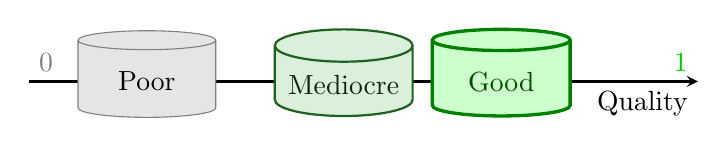
\begin{tikzpicture}
	[basket/.style={cylinder, shape border rotate=90,aspect=0.25, minimum height=1.1cm,minimum width=1.75cm},
	poor/.style={basket, draw=gray, fill=gray!20!white},
	mediocre/.style={basket, thick, green!30!gray!20!black, draw=green!50!gray!50!black, fill=green!40!gray!20!white},
	good/.style={basket, very thick, green!30!black, draw=green!50!black, fill=green!20!white}]

\draw [->,thick,draw=,>=stealth] (-2,0) node [above right,gray] {0} -- (6.5, 0) node [above left,green!80!black] {1} node [below left,black] {Quality};
\node [poor] at (-0.5,0.0) {Poor};
\node [mediocre] at (2.0,-0.05) {Mediocre};
\node [good] at (4.0,0.0) {Good};

\end{tikzpicture}
\end{document}
